\begin{activity} \label{A:11.7.1} Suppose our box $B$ has the form $[a,b] \times [c,d] \times [r,s]$, that is $B = \{(x,y,z) : a \leq x \leq b, c \leq y \leq d, r \leq z \leq s\}$. We partition the box as illustrated in Figure \ref{F:11.7.Box_domain_2}.

\begin{figure}[ht]
\begin{center}
%\resizebox{!}{2.0in}{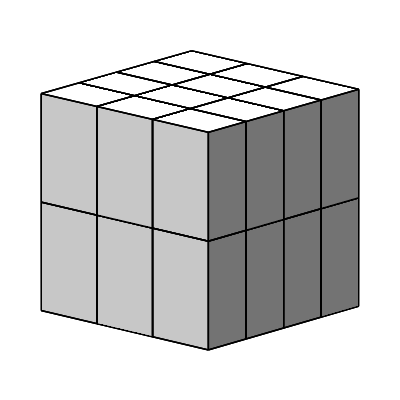
\includegraphics[trim=0cm 1.5cm 0cm 1.5cm, clip]{11_7_Box_domain_2}}
  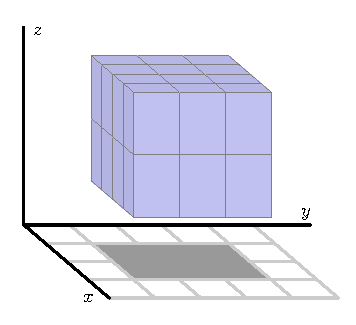
\includegraphics{figures/fig_11_7_partition.eps}
\end{center}
\caption{A partitioned three-dimensional domain.}
\label{F:11.7.Box_domain_2}
\end{figure}
%crop graphics in animate trim=<left> <bottom> <right> <top>, clip with includegraphics
	\ba
	\item Let $a=x_0 < x_1 < x_2 < x_3 < x_4=b$ be the endpoints of the subintervals of $[a,b]$ after partitioning. Label these endpoints in Figure \ref{F:11.7.Box_domain_2}. What is the length $\Delta x$ of each subinterval $[x_{i-1},x_i]$ for $i$ from 1 to 4? Your answer should be in terms of $a$ and $b$.
	
	
		
	\item Let $c=y_0 < y_1 < y_2 < y_3=d$ be the endpoints of the subintervals of $[c,d]$ after partitioning. Label these endpoints in Figure \ref{F:11.7.Box_domain_2}. What is the length $\Delta y$ of each subinterval $[y_{j-1},y_j]$ for $j$ from 1 to 3? Your answer should be in terms of $c$ and $d$.
	
	

	\item Let $r=z_0 < z_1 < z_2=s$ be the endpoints of the subintervals of $[r,s]$ after partitioning. Label these endpoints in Figure \ref{F:11.7.Box_domain_2}. What is the length $\Delta z$ of each subinterval $[z_{k-1},z_k]$ for $k$ from 1 to 2? Your answer should be in terms of $r$ and $s$.
	
	

	\item The partitions of the intervals $[a,b]$, $[c,d]$, and $[r,s]$ partition the box $B$ into sub-boxes. How many sub-boxes are there? What is the volume $\Delta V$ of each sub-box?
	
	
	
	\item Let $B_{ijk}$ denote the sub-box $[x_{i-1},x_i] \times [y_{j-1},y_j] \times [z_{k-1},z_k]$. Label each visible sub-box in Figure \ref{F:11.7.Box_domain_2}.
	
	
	
	
	\item Now let $(x_{ijk}^*, y_{ijk}^*, z_{ijk}^*)$ be an arbitrary point in the $i,j,k$th sub-box. Explain what the product
\[\delta(x_{ijk}^*, y_{ijk}^*, z_{ijk}^*) \Delta V\]
represents.



    \item If we were to add all the values $\delta(x_{ijk}^*, y_{ijk}^*, z_{ijk}^*) \Delta V$ for each $i$, $j$, and $k$, what does the resulting number approximate about the piece of granite?

	
	
	\item Write a triple sum using summation notation that expresses the arbitrary sum from part (k).
		
	
	\ea

\end{activity}
\begin{smallhint}

\end{smallhint}
\begin{bighint}

\end{bighint}
\begin{activitySolution}
	\ba
	\item The endpoints are labeled in the figure below. Since we are partitioning the interval $[a,b]$ into 4 subintervals of equal length, the length of each subinterval is $\Delta x = \frac{b-a}{4}$. 	
		
	\item The endpoints are labeled in the figure below. Since we are partitioning the interval $[c,d]$ into 3 subintervals of equal length, the length of each subinterval is $\Delta y = \frac{d-c}{3}$. 	

	\item The endpoints are labeled in the figure below. Since we are partitioning the interval $[r,s]$ into 2 subintervals of equal length, the length of each subinterval is $\Delta z = \frac{s-r}{2}$.

	\item The total number of sub-boxes is $4 \times 3 \times 2 = 24$. The volume of each sub-box is $\Delta V = \Delta x \ \Delta y \ \Delta z$. 
		
	\item The visible sub-boxes are shown in the figure below. 
	
	\item We are assuming a constant density of $\delta(x_{ijk}^*, y_{ijk}^*, z_{ijk}^*)$ in the sub-box $B_{ijk}$, so the product 
\[\delta(x_{ijk}^*, y_{ijk}^*, z_{ijk}^*) \Delta V\]
approximates the mass of the sub-box $B_{ijk}$.

    \item Since each $\delta(x_{ijk}^*, y_{ijk}^*, z_{ijk}^*) \Delta V$ approximates the mass of a sub-box, if we add all the values for each $i$, $j$, and $k$, the sum will approximate the mass of this piece of granite.
	
	\item A triple sum using summation notation that expresses the arbitrary sum from part (k) is
\[\sum_{k=1}^2 \sum_{j=1}^3 \sum_{i=1}^4 \delta(x_{ijk}^*, y_{ijk}^*, z_{ijk}^*) \Delta V.\]
		
	
	\ea
%\begin{figure}[h]
\begin{center}
%\resizebox{!}{2.0in}{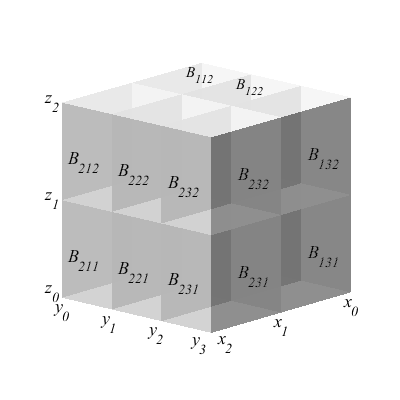
\includegraphics[trim=0cm 1.5cm 0cm 1.5cm, clip]{11_7_1_box_labeling.png}}
\end{center}
%\caption{A partitioned three-dimensional domain.}
%\label{F:11.7.Box_domain_2}
%\end{figure}
\end{activitySolution}
\aftera
